% mnras_template.tex 
%
% LaTeX template for creating an MNRAS paper
%
% v3.0 released 14 May 2015
% (version numbers match those of mnras.cls)
%
% Copyright (C) Royal Astronomical Society 2015
% Authors:
% Keith T. Smith (Royal Astronomical Society)

% Change log
%
% v3.0 May 2015
%    Renamed to match the new package name
%    Version number matches mnras.cls
%    A few minor tweaks to wording
% v1.0 September 2013
%    Beta testing only - never publicly released
%    First version: a simple (ish) template for creating an MNRAS paper

%%%%%%%%%%%%%%%%%%%%%%%%%%%%%%%%%%%%%%%%%%%%%%%%%%
% Basic setup. Most papers should leave these options alone.
\documentclass[fleqn,usenatbib,]{mnras}
\usepackage{lineno}
\linenumbers
% MNRAS is set in Times font. If you don't have this installed (most LaTeX
% installations will be fine) or prefer the old Computer Modern fonts, comment
% out the following line
\usepackage{newtxtext,newtxmath}
% Depending on your LaTeX fonts installation, you might get better results with one of these:
%\usepackage{mathptmx}
%\usepackage{txfonts}

% Use vector fonts, so it zooms properly in on-screen viewing software
% Don't change these lines unless you know what you are doing
\usepackage[T1]{fontenc}
\usepackage{ae,aecompl}


%%%%% AUTHORS - PLACE YOUR OWN PACKAGES HERE %%%%%

% Only include extra packages if you really need them. Common packages are:
\usepackage{graphicx}	% Including figure files
\usepackage{amsmath}	% Advanced maths commands
\usepackage{amssymb}	% Extra maths symbols
\usepackage{booktabs}   % Make tables directly in pandas
\usepackage{longtable}  % Add longer tables
\usepackage{rotating}
\usepackage{appendix}
\usepackage{float}
\usepackage[dvipsnames]{xcolor}
\usepackage{subcaption}
\usepackage{multicol}
\usepackage{wrapfig}
\PassOptionsToPackage{hyphens}{url}\usepackage{hyperref}
\captionsetup{compatibility=false}

\setlength{\rotFPtop}{0pt plus 1fil}% <- add this line after loading rotating
\setlength{\rotFPbot}{0pt plus 1fil}% <- maybe its better to add this line too
\usepackage{threeparttable}
\makeatletter
%\newlength{\abovecaptionskip}%
%\setlength{\abovecaptionskip}{10\p@}
\makeatother
\usepackage{booktabs}
%%%%%%%%%%%%%%%%%%%%%%%%%%%%%%%%%%%%%%%%%%%%%%%%%%

%%%%% AUTHORS - PLACE YOUR OWN COMMANDS HERE %%%%%

% Please keep new commands to a minimum, and use \newcommand not \def to avoid
% overwriting existing commands. Example:
%\newcommand{\pcm}{\,cm$^{-2}$}	% per cm-squared
%Co-authors:
\newcommand{\phil}[1]{\color{red}#1 \color{black}}

\newcommand{\comment}[1]{\textbf{[#1]}} %comments

%define some nice astro shortcuts
\newcommand{\halpha}[0]{H$\alpha$}
\newcommand{\hbeta}[0]{H$\beta$}
\newcommand{\OII}[0]{$[\textnormal{\textsc{Oii}}]$}
\newcommand{\OIII}[0]{$[\textnormal{\textsc{Oiii}}]$}
\newcommand{\SII}[0]{$[\textnormal{\textsc{Sii}}]$}
\newcommand{\SIII}[0]{$[\textnormal{\textsc{Siii}}]$}
\newcommand{\NII}[0]{$[\textnormal{\textsc{Nii}}]$}
\newcommand{\msun}[0]{M_{\odot}}


\defcitealias{Pursiainen2018}{P18}
\defcitealias{Pursiainen2020}{P20}
%%%%%%%%%%%%%%%%%%%%%%%%%%%%%%%%%%%%%%%%%%%%%%%%%%
%This if a fix from https://tex.stackexchange.com/questions/249579/pdfendlink-ended-up-in-different-nesting-level-than-pdfstartlink-error-with/249743#249743 to sort hyperref breaking in pdfendlink when a reference spills over a page
%\usepackage{etoolbox}
%\makeatletter
%\patchcmd\@combinedblfloats{\box\@outputbox}{\unvbox\@outputbox}{}{%
%  \errmessage{\noexpand\@combinedblfloats could not be patched}%
%}%
%\makeatother
%
%\defcitealias{Smith2019}{S19}
%\defcitealias{Kelly2012}{KK12}
%%%%%%%%%%%%%%%%%%% TITLE PAGE %%%%%%%%%%%%%%%%%%%

% Title of the paper, and the short title which is used in the headers.
% Keep the title short and informative.
\title[Supernova hosts in DES]{Supernova Host Galaxies in the Dark Energy Survey: \\ II. Rapidly Evolving Transients}
% The list of authors, and the short list which is used in the headers.
% If you need two or more lines of authors, add an extra line using \newauthor
\author[P. Wiseman et al.]{
P. Wiseman$^1$\thanks{E-mail: p.s.wiseman@soton.ac.uk (PW)},
 M. Pursiainen$^1$,
 M. Smith$^1$,
 M. J. Childress$^1$,
 and Other Authors$^{1,2}$,
\newauthor
(The DES Collaboration)
\\
% List of institutions
$^{1}$School of Physics and Astronomy, University of Southampton, Southampton, SO17 1BJ, UK\\
$^{2}$Other Institutions\\
%$^{3}$Another Department, Different Institution, Street Address, City Postal Code, Country
}

% These dates will be filled out by the publisher
\date{Accepted XXX. Received YYY; in original form ZZZ}

% Enter the current year, for the copyright statements etc.
\pubyear{2020}
% These dates will be filled out by the publisher

% Don't change these lines
\begin{document}
\label{firstpage}
\pagerange{\pageref{firstpage}--\pageref{lastpage}}
\maketitle

% Abstract of the paper
\begin{abstract}
Rapidly evolving transients (RETs) are a mysterious class of astrophysical event. They are characterised by lightcurves that decline much faster than standard supernovae (SNe), span vast ranges in peak luminosity and can be seen to redshifts greater than 1. 
\end{abstract}

% Select between one and six entries from the list of approved keywords.
% Don't make up new ones.
\begin{keywords}
keyword1 -- keyword2 -- keyword3
\end{keywords}

%%%%%%%%%%%%%%%%%%%%%%%%%%%%%%%%%%%%%%%%%%%%%%%%%%

%%%%%%%%%%%%%%%%% BODY OF PAPER %%%%%%%%%%%%%%%%%%

\section{Introduction}



In the standard paradigm of stellar evolution, stars with a zero-age main sequence (ZAMS) mass above $8M_{\sun}$ are believed to explode as a result of a catastrophic collapse of their iron cores and are known as core-collapse supernovae (CCSNe). Since the turn of the century, observations of CCSNe, whose lightcurves are primarily powered by the radioactive decay of freshly synthesised Ni-56, have been supplemented by rarer, more exotic transient classes.

 Long duration gamma-ray bursts (LGRBs), although first discovered in the 1960s \citep{Klebesadel1973} were only unequivocally linked to collapsing massive stars their associations with broad-lined type Ic SNe \citep{Galama1998,Hjorth2003}. Thought to be caused by accretion onto a newly-formed black hole at the centre of a collapsing, rapidly-rotating massive star \citep[][e.g.]{Woosley1993,Woosley2006a,Woosley2006b}, LGRBs comprise roughly $1\%$ of all SNe Ic, themselves making up only 15\% of all CCSNe \citep{Kelly2012,Graham2016}. The second exotic class of SNe is the particularly bright superluminous supernovae (SLSNe; e.g. \citealt{Quimby2011, Gal-Yam2012}). Originally grouped due to their slowly-evolving lightcurves and extreme luminosity (peaking at $M_B < -21$~mag), recent observations have revealed a continuum of spectroscopically similar objects with peaks as faint as $M_B \sim -19$~mag \citep{DeCia2018,Lunnan2018,Angus2019}, similar to the bright end of the CCSN luminosity function \citet{Li2010,Grayling2020}. The lightcurve evolution of SLSNe is not well described by models of Ni-56 decay, with the most popular alternative hypothesis being the magnetic coupling of the ejecta with the spin down of a newly-formed magnetar.
 
 Along with observations of the transients themselves, host galaxies are frequently-used laboratories from which strong inferences about the progenitor stars and explosion mechanisms can be made. Core-collapse SNe are confined almost exclusively to galaxies hosting recent or ongoing star formation, due to their origin from massive stars. There are correlations between the expected progenitor mass of different sub-classes of CCSNe and host galaxy properties. On average, stripped envelope SNe (SESNe; types Ib, Ic and their sub-types) reside in galaxies with higher specific star-formation rate (sSFR) and younger stellar age \citep{Galbany2018}, indicating that their progenitors are more massive than the various sub-classes of hydrogen-rich SNe II.
 
 Metallicity is an important consideration when comparing host galaxy properties. While it does not appear to play a significant role in the relative production of CCSNe (although there are some trends, with SESNe typically found in slightly less metal-rich galaxies than SNe II), it appears to be vitally important in the production of LGRBs and SLSNe. Theory predicts that the production of a LGRB should only be possible in stars with a metallicity of $Z/Z_{\sun}\leq 0.3$ \citep{Woosley1993}  in order for the likely Wolf-Rayet or blue supergiants progenitors not to lose their outer atmospheres through metal-driven winds, thus conserving sufficient angular momentum to power the black-hole-driven jet or rapidly rotating magnetar. Many LGRB host galaxy studies have indeed revealed a metallicity threshold to be observed between 0.5 and 1 times the solar value \citep[e.g.][]{Stanek2006,Modjaz2008,Kruehler2015,Perley2016b,Japelj2016,Vergani2017}.  
SLSN host galaxies also appear to be lower in metallicity than would be expected for their stellar mass, with a suppression of SLSN production at a value around half-solar \citep{Lunnan2014,Chen2016a,Perley2016c}. They also require particularly high sSFR, suggesting that they are explosions of very young, rapidly rotating massive stars.
 
Recently, inspection of high-cadence, all-sky survey data sets have revealed yet more exotic transients that are less easy to explain with conventional models. \citet{Drout2014} revealed a class of rapidly evolving transients (RETs) in the Pan-STARRS survey (PS1). \citet{Pursiainen2018} expanded the known number of RETs to beyond 80 with their sample from the Dark Energy Survey (DES), spanning a redshift range of $\sim 0$ to $>1$. RETs typically rise to peak brightness within 7-10 days, and decline to 10\% of their peak brightness within 30 days, much faster than typical SNe. The photometric measurements of the PS1 and DES RETs seem to be well described by simple expanding blackbodies, although a handful show declining photospheric radii from the outset. Due to the rapid nature of their lightcurves and location at high-redshift, spectral coverage is sparse and signal-to-noise ratio (SNR) is low, such that there has not yet been a conclusive detection of absorption or emission features from the transients. 

There are a limited number of local analogues to the RETs seen in the samples of PS1 and DES at cosmological distances, the most widely studied of which is AT2018cow \citep[e.g.]{Prentice2019,Lyman2019,Perley2019}. The transient declined from its discovery, with constraints on a ~1 day rise time, and did not resemble any known SN, GRB afterglow, or kilonova (KN). 
Other nearby rapid transients include the local fast-declining SN Ibn SN2018kzr \citep{McBrien2020}, and KSN-2015K \citep{Rest2018}. It is currently unclear whether these transients 

In this paper, we present the first comprehensive study of the host galaxies of rapidly evolving transients. We make use of the final DES sample, which builds on \citet{Pursiainen2018} using the final year of data as well as more refined discovery techniques. Using the deep DES photometry from \citet{Wiseman2020} and spectra from OzDES \citep{Lidman2020} we derive host galaxy properties in order to compare them to samples of CCSNe, LGRBs, and SLSNe. 

The order of the paper is as follows:
Where applicable, we adopt a spatially flat $\Lambda$CDM cosmology with the parameters H$0=70$ km~s$^{-1}$ and $\Omega_{\textrm{M}}=0.3$.



\section{Sample selection\label{sec:sample}}

We derive our sample from the 106 RETs discovered in the 5-year DES-SN transient survey. This number expands upon the 72 of \citetalias{Pursiainen2018} and is presented in a companion work \citetalias{Pursiainen2020}. We refer to the full sample as DES RETs. In order to calculate host galaxy properties Of the 106 objects in the sample, \textbf{n} have a host galaxy detected in deep host galaxy photometry (Section \ref{sec:obs}), of which 49 have a host galaxy spectroscopic redshift. A further two have redshifts 

\subsection{Comparison samples \label{subsec:comparison}}

In order to compare the host galaxies of DES RETs to those discovered in other surveys as well as other types of explosive transient, we draw upon samples in the literature. 

\subsubsection{RETs \label{subsubsec:compare_rets}}
Since the DES sample of RETs is by far the largest discovered to date, there is no other large sample of RETs with which to compare host galaxy properties. \citet{Drout2014} present host galaxies of 10 RETs discovered in the Pan-STARRS survey, with measurements of stellar masses and SFRs. To this we add the low-redshift transients AT2018cow \citep[e.g.][], with host galaxy measurements from \citet{Perley2019} (Metallicity??), and SN2018kzr (measurements??).

\subsubsection{SNe and GRBs \label{subsubsec:compare_CCSNe}}

To compare with CCSNe, we draw on the PMAS/PPak Integral-field Supernova hosts COmpilation (PISCO) sample presented in \citet{Galbany2018}. 

We use the sample of GRB host galaxies of \citet{Kruehler2015}, using only galaxies with $z<1$ in order to maintain completeness. 

To investigate similarities with CCSNe, we use the PTF sample of \citet{Perley2016c}






\section{Host galaxy observations \label{sec:obs}}
\subsection{Photometry \label{subsec:phot}}

The host galaxy photometry for the sample of RETs is taken from the catalogue of \citet{Wiseman2020}, which is based upon deep coadds reaching $r$-band limiting magnitudes of 26.5. The coadds were created using data from all five seasons of DES-SN, but by excluding one season at a time in order for that coadd not to include contamination from the transients in that season. For this sample, the limiting magnitude for obtaining a spectroscopic redshift (\ref{subsec:spec}) is $\sim 24.5$, meaning that all hosts in the sample are detected with a high S/N.

\subsection{Spectroscopy \label{subsec:spec}}
Accurate redshifts for DES-SN were obtained by OzDES\footnote{Australian (Oz) Dark Energy Survey}, a dedicated DES spectroscopic follow-up campaign based at the $3.9~\textrm{m}$ Anglo-Australian Telescope (AAT) using the AAOmega fibre-fed spectrograph and 2dF fibre positioner. The observation strategy of OzDES was to point at one of the ten DES-SN fields, and place fibres at the positions of transient hosts, continually coadding the spectra of a particular host until a redshift was obtained at which point the fibre could be allocated to a different transient. The spectra have a resolution of 1400-1700 and a wavelength range of 3700$\AA - 8800\AA$, and are reduced using a modified version of 2dfdr \citep{Croom2004} along with internal scripts. Extensive description and discussion of OzDES can be found in \citet{Yuan2015,Childress2017,Lidman2020}.

\section{Estimating host galaxy properties \label{sec:measure}}

\subsection{SED fitting \label{subsec:sedfit}}

To estimate the physical properties of the host galaxies, we generate synthetic photometry in the DES $griz$ bands by combining the individual SEDs of simple stellar population models. 

\subsection{Spectral line fitting \label{subsec:linefit}}

To estimate parameters from the OzDES host galaxy spectra requires several processing steps. We first apply a flux calibration using the method of \citet{Swann2020}, by `mangling' the spectrum such that the integrated flux over the wavelength ranges of the DES photometric bands matches that measured in the photometry. Rather than using global galaxy photometry (i.e. using a Kron aperture), we use a circular aperture of diameter 2\arcsec, matching the size of the spectrograph fibres.  

In order to subtract the stellar component of the host galaxy spectra, we use the Penalized PiXel-Fitting software (\texttt{pPXF}; \citealt{Cappellari2004,Cappellari2012,Cappellari2017}), using the MILES library of single stellar populations \citep{Vazdekis2010}. By subtracting the best-fitting stellar spectrum from the \texttt{pPXF} fit, we are left with a `gas' spectrum, comprising the emission lines. We fit the emission lines using \texttt{PySpecKit} \citep{Ginsburg2011}. In order to estimate the uncertainty on the emission line fluxes, we fit $10^4$ realisations of the line, each time adding a perturbation to the amplitude of the line by drawing from a Gaussian distribution centered on 0, and with a standard deviation equal to the root-mean-square (RMS) of the measured flux noise in that part of the spectrum. We take the mean and standard deviation of the resulting fits as our flux and its uncertainty, respectively.

\subsection{Estimating metallicities \label{subsec:calc_Z}}

The most common method used to estimate the metallicity of galaxies is to use emission line ratios that have been calibrated using theoretical or empirical models in order to approximate the gas-phase oxygen abundance in the interstellar medium. Due to the low S/N of the spectra in this sample, we are constrained to a subset of these diagnostics by the availability of only a handful of the strongest emission lines, namely \halpha, \hbeta, \OII 3727, \OIII 4959 and 5007, \NII 6548 and 6583, and \SII 6717 and 6731. Furthermore, for each host galaxy only a subset of these lines are detected - for example, \halpha, \NII and \SII are redshifted out of the spectral coverage at $z>0.3$, leaving only the oxygen lines available, mandating the use of the R23 diagnostic. For hosts at $z<0.3$ we are able to use the \OIII /\NII (O3N2) and \NII /\halpha (N2) line ratios. 

For the R23 indicator, we use the calibration of \citet{Pettini2004} (PP04), while for O3N2 and N2, we use the calibration of \citet{Marino2013} (M13) in order to directly compare metallicity with the Pisco CCSN sample. We recalculate the metallicities given in \citet{Kruehler2015} using the M13 calibration. 


\begin{figure}
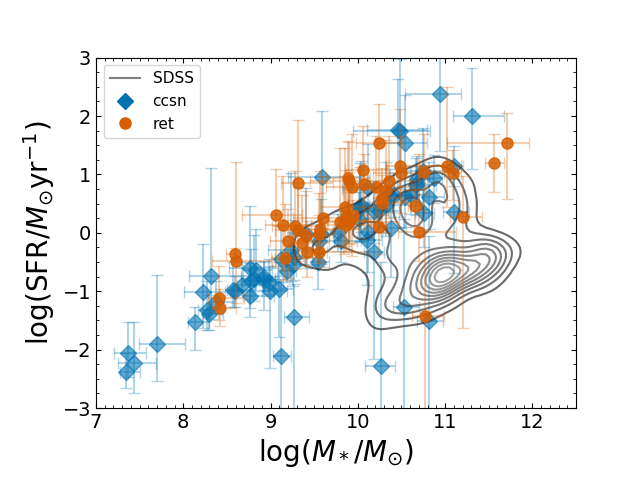
\includegraphics[width=0.5\textwidth]{figs/SFR_Mike.png}
\caption{The SFR of RET hosts, compared to CCSNe and the low-z SDSS sample.
\label{fig:sfms_sfr}}
\end{figure}

\begin{figure}
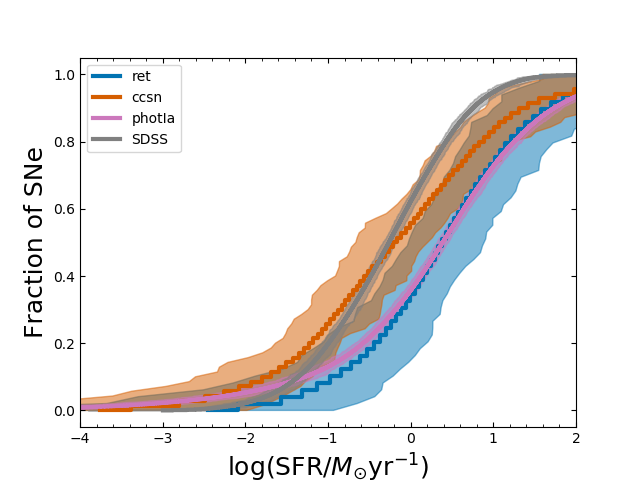
\includegraphics[width=0.5\textwidth]{figs/cum_SFR_mike.png}
\caption{Cumulative distributions of the SFR of RET hosts, compared to CCSNe and the low-z SDSS sample.
\label{fig:sfr_cum}}
\end{figure}

\begin{figure}
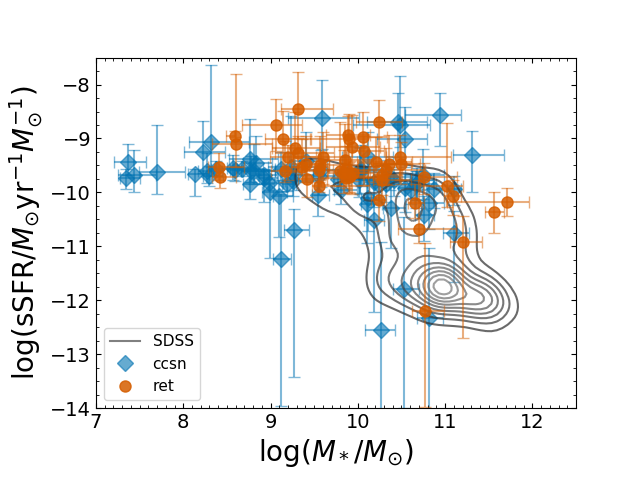
\includegraphics[width=0.5\textwidth]{figs/sSFR_Mike.png}
\caption{The sSFR of RET hosts, compared to CCSNe and the low-z SDSS sample.
\label{fig:sfms_ssfr}}
\end{figure}

\begin{figure}
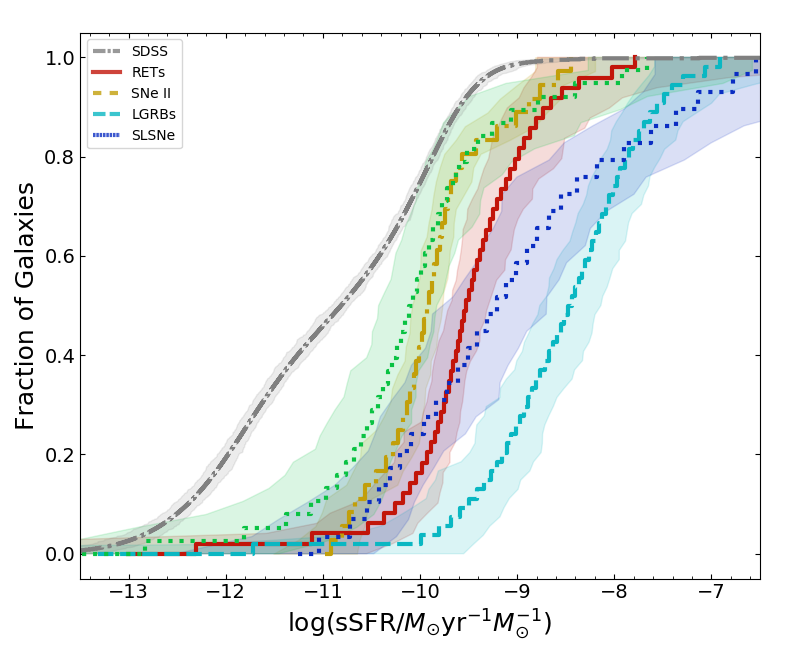
\includegraphics[width=0.5\textwidth]{figs/cum_sSFR_mike.png}
\caption{Cumulative distributions of the sSFR of RET hosts, compared to CCSNe and the low-z SDSS sample.
\label{fig:ssfr_cum}}
\end{figure}


\section{Analysis and Discussion}
\label{sec:analysis} % used for referring to this section from elsewhere



\subsection{Stellar Mass \label{subsec:res_mass}}

\subsection{Star formation rate \label{subsec:res_sfr}}
Fig.~\ref{fig:sfms_sfr} shows the `star formation main sequence' (SFMS) of RET host galaxies along with that for CCSNe and for the field galaxies of SDSS. RETs and CCSNe both systematically avoid passive galaxies, suggesting that RETs may require the presence of star-formation and thus be linked to massive stars.

In Fig.~\ref{fig:sfr_cum} we show the cumulative distributions of the star-formation rate in RETs, CCSNe, and SDSS galaxies. With the exception of three objects, all RETs occured in galaxies with $\textrm{SFR}>0.1 \msun$yr$^{-1}$, and the curve is shifted towards higher SFRs than that for CCSNe. This would imply that a higher SFR is required for RETs to occur - or can be thought of as a higher SFR threshold for the formation of a RET progenitor.

Fig.~\ref{fig:sfms_ssfr} is similar to Fig.~\ref{fig:sfms_sfr}, except that here SFR has been normalised by stellar mass, and thus shows the specific star-formation rate (sSFR), which is more representative measure of the star-forming nature of the galaxy itself. It is once again clear that RET hosts lie systematically above the majority of SDSS star-forming galaxies. Normalised by mass, it is here perhaps clearer to see that RET hosts lie at higher sSFR than CCSNe hosts.

As for SFR, we show the cumulative distribution of sSFR in Fig.~\ref{fig:ssfr_cum}. The RET hosts are clearly shifted higher sSFRs than CCSNe. This result is significant as there are no obvious selection effects which could cause the shift.

\subsection{Metallicity \label{subsec:res_metallicity}}
\begin{figure}
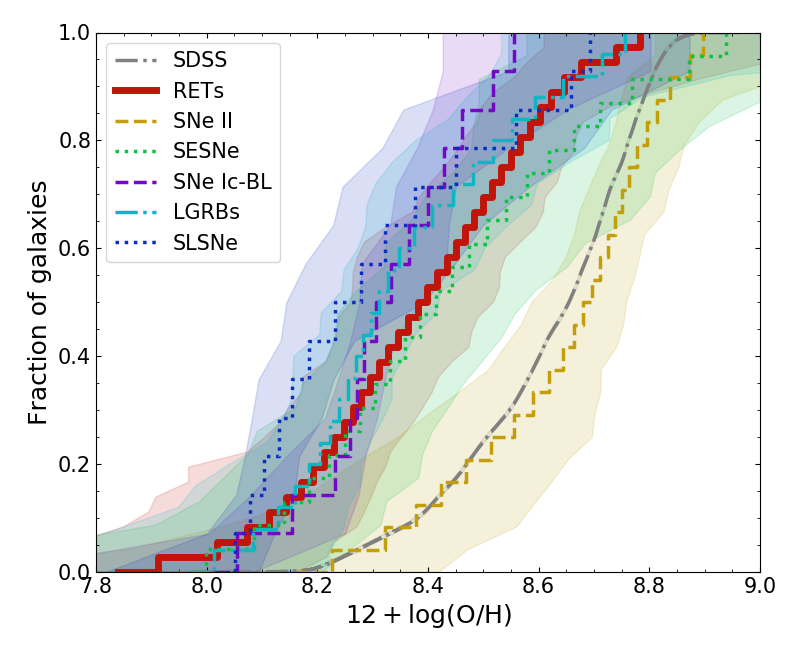
\includegraphics[width=0.5\textwidth]{figs/RET_OH_cum.png}
\caption{Cumulative distributions of the gas-phase oxygen abundances of RET hosts, compared to CCSNe and the low-z SDSS sample.
\label{fig:oh_cum}}
\end{figure}

\begin{figure*}
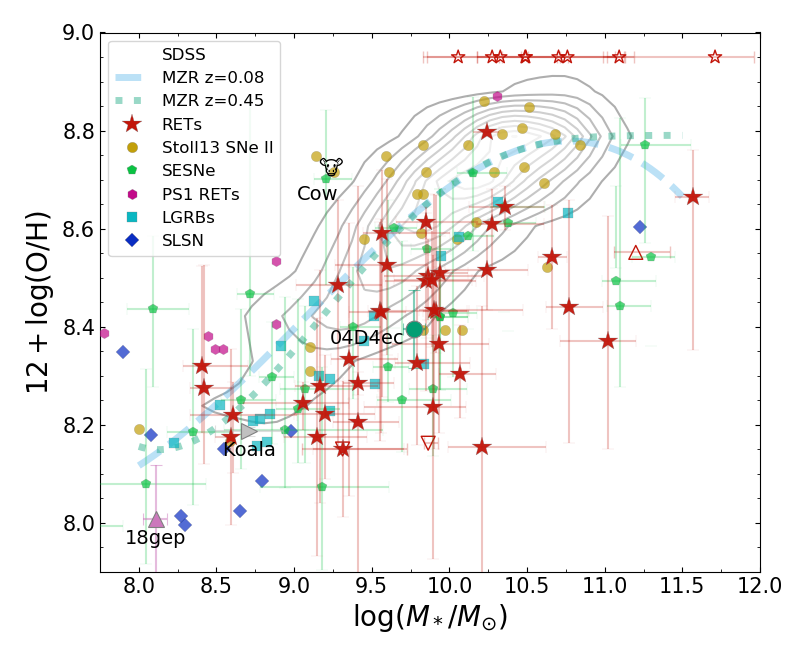
\includegraphics[width=\textwidth]{figs/RET_MZR.png}
\caption{The mass-metallicity relation (MZR) for RET host galaxies.
\label{fig:mzr}}
\end{figure*}

In the Section \ref{subsec:res_sfr} we demonstrate that RETs occur in galaxies with systematically higher sSFR than CCSNe, to which one explanation is that they are related to more massive stars. A further property that could directly impact the composition of stellar populations harbouring potential RET progenitors is the metallicity. Using the gas-phase oxygen abundances calculated in Section \ref{subsec:calc_Z} as a proxy for metallicity, we can compare the chemical state of RET host galaxies with CCSNe and star-forming field galaxies. The cumulative distributions of metallicity are displayed in \ref{fig:oh_cum}, and show RET hosts to be consistent with CCSNe and field galaxies. While the RET curve lies at lower metallicity than CCSNe and field galaxies in the $8.4 < \log \left(12+\textrm{O/H}\right)<9.0$ range, this is entirely within the $1\sigma$ uncertainty region for the RET host CDF. In Fig.~\ref{fig:mzr} we show the mass-metallicity relation (MZR) for the RET and comparison samples.



\section{Discussion \label{sec:disc}}

\subsection{Transient - host galaxy correlations}



\section{Conclusions}

The last numbered section should briefly summarise what has been done, and describe
the final conclusions which the authors draw from their work.

\section*{Acknowledgements}

The Acknowledgements section is not numbered. Here you can thank helpful
colleagues, acknowledge funding agencies, telescopes and facilities used etc.
Try to keep it short.

%%%%%%%%%%%%%%%%%%%%%%%%%%%%%%%%%%%%%%%%%%%%%%%%%%

%%%%%%%%%%%%%%%%%%%% REFERENCES %%%%%%%%%%%%%%%%%%

% The best way to enter references is to use BibTeX:

\bibliographystyle{mnras}
\bibliography{PhilMendeley} % if your bibtex file is called example.bib


% Alternatively you could enter them by hand, like this:
% This method is tedious and prone to error if you have lots of references
%\begin{thebibliography}{99}
%\bibitem[\protect\citeauthoryear{Author}{2012}]{Author2012}
%Author A.~N., 2013, Journal of Improbable Astronomy, 1, 1
%\bibitem[\protect\citeauthoryear{Others}{2013}]{Others2013}
%Others S., 2012, Journal of Interesting Stuff, 17, 198
%\end{thebibliography}

%%%%%%%%%%%%%%%%%%%%%%%%%%%%%%%%%%%%%%%%%%%%%%%%%%

%%%%%%%%%%%%%%%%% APPENDICES %%%%%%%%%%%%%%%%%%%%%

\appendix

\section{Some extra material}

If you want to present additional material which would interrupt the flow of the main paper,
it can be placed in an Appendix which appears after the list of references.

%%%%%%%%%%%%%%%%%%%%%%%%%%%%%%%%%%%%%%%%%%%%%%%%%%


% Don't change these lines
\bsp	% typesetting comment
\label{lastpage}
\end{document}

% End of mnras_template.tex